\chapter{Selección de eventos}

\section{Trigger}\label{sec:trigger}

Como se menciono en la sec los datos fueron colectados utilizando un trigger
de un fotón (\trigchain), que selecciona eventos con al menos un fotón loose con
momento transverso mayor a 120 \gev.
La eficiencia de este trigger fue calculada y es de $100^{+0}_{-1.41}$(stat)${}^{+0}_{-0.7}$(syst) \%,
con respecto a candidatos a fotones aislados con $\pt>125 \gev$.
%%Los detalles del calculo de la The details of this calculation are discussed in \cref{sec:trigger_eff}.

La eficiencia del trigger fue calculada utilizando un método bootstrap siguiendo las prescripciones
xsdescriptas en \cref{Damazio:1609629} y se puede ver el resultado como función del {\pt} y $\eta$ del
fotón en la \cref{fig:trigger_perf}.

\begin{figure}[h!]
  \centering
  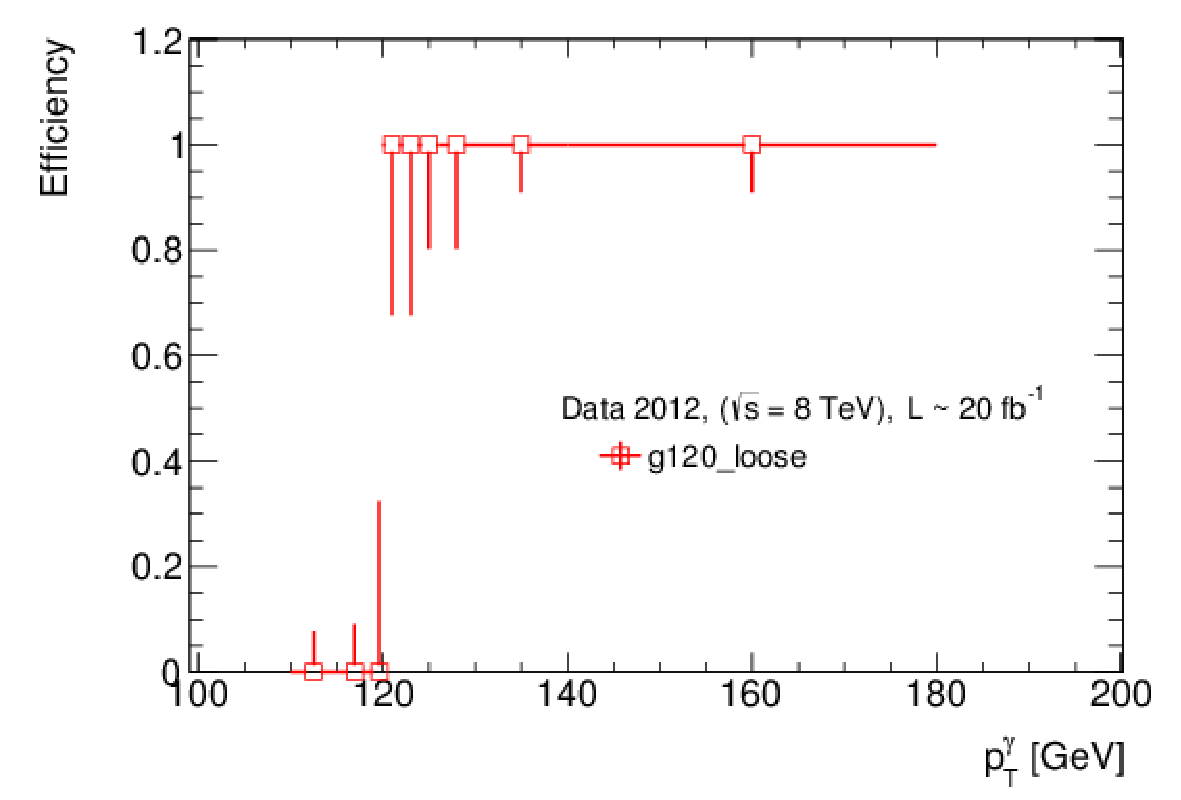
\includegraphics[width=0.49\textwidth]{figures/EffPtg120_loose}
  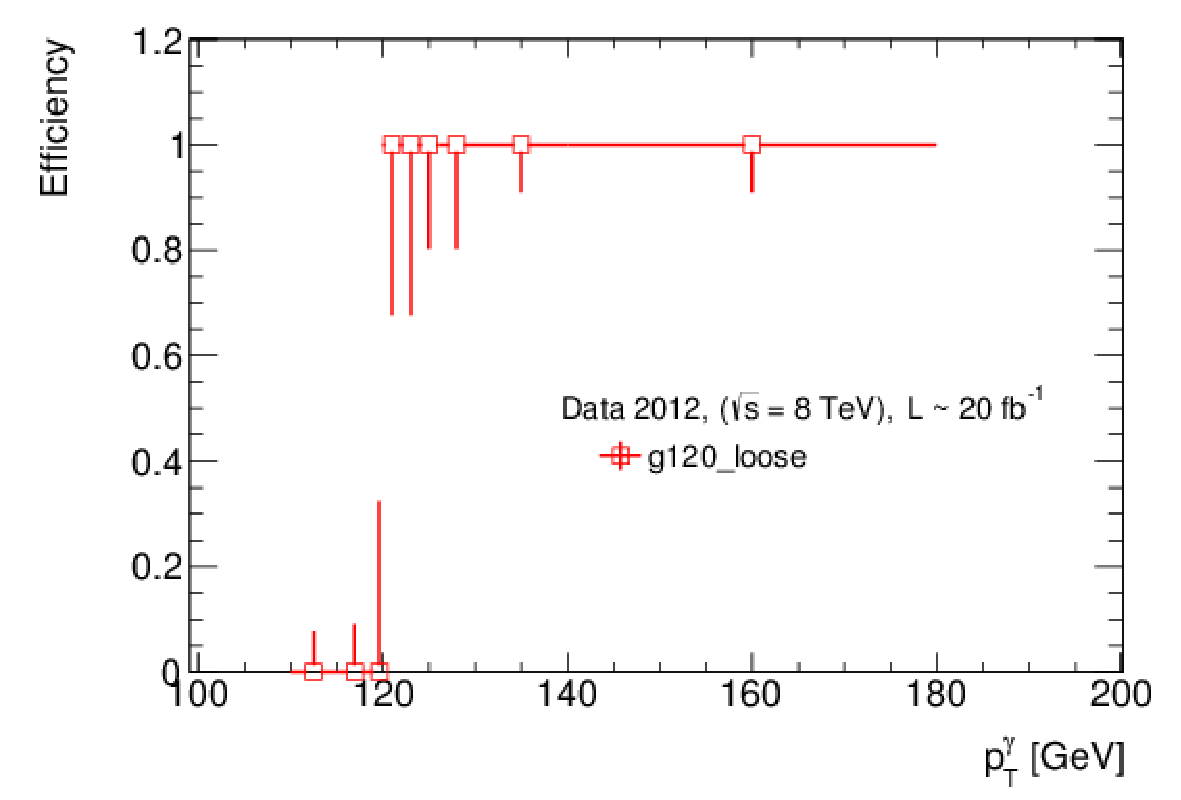
\includegraphics[width=0.49\textwidth]{figures/EffPtg120_loose}
  \caption{Eficiencia del trigger para {\trigchain} como función del {\pt} del fotón (izquierda)
    y $\eta$ (derecha).}\label{fig:trigger_perf}
\end{figure}


\section{Preselección}\label{sec:base_seleccion}

Antes de aplicar los cortes cinemáticos, se realiza la siguiente
preselección y limpieza tanto para la regiones de señal como las de control.

\begin{itemize}\itemsep0.1cm
\item[-] Data quality (GRL) and single photon trigger, as described in \cref{sec:trigger}.
%	The events must be accepted by the GoodRunList (only for data) and single photon trigger selection as described in \cref{sec:datasamples}
\item[-] Primary vertex:
The vertex candidates for the $pp$ interactions in each event are reconstructed from the ID tracks. The
primary vertex, corresponding to the hard scattering interaction, is the vertex candidate with the largest
sum of $p_{T}^{2}$ for the associated tracks. Events with at least five charged tracks associated to the primary
vertex are selected.
\item[-] Data quality: for data samples only, cleaning from noise bursts in the calorimeters and possible incomplete events due to the TTC reset procedure is applied. Events must
have %%|larError==0|, \verb|tileError==0|, and \verb|(coreFlags&0x4000)==0|.
\end{itemize}

La selección de los objetos se realiza según lo descripto en \cref{sec:obj_selection}.
El overlap removal y el event veto aplicado se detalla en la \cref{sec:overlap_romoval_event_veto}.

\section{Optimización de las regiones de se\~nal}

Se dividió el análisis en dos regiones de señal, {\SRL} y {\SRH}.
La primera optimizada para gluinos de alta masa acompañados por el decaimiento de
neutralinos NLSP de baja y moderada mada. Esta se caracteriza por un gran multiplicad
de jets y actividad hadronica, debido a que involucra cadenas de decaimiento largas de gluinos
pesados a través de producción de charginos.

La segunda región tiene como motivación los escenarios mas compressed donde la masa de los gluinos
y del neutralino están cerca una de la otra. La cadena de decaimiento es por lo tanto mucho mas corta
en este caso, con menor numero de jets, fotones de alto pt y gran cantidad de met en el estado final.

Los puntos benchmark generados en el plano de masa de gluino/neutralino para cada SR se muestran en la
\cref{fig:SRegions}.

Para la optimización de la selección de eventos, se asume una luminosidad total integrada de
$20.3~\ifb$ y una incerteza en la estimación del fondo del {\SM} del 25\%. La significance
utilizada en la optimización se define como:

\begin{equation*}
  Z_A = \sqrt{2 \left( (s + b) \log\left[\frac{(s + b) (b + \sigma_b^2)}{b^2 + (s + b) \sigma_b^2}\right] - \frac{b^2}{\sigma_b^2} \log\left[1 + \frac{s \sigma_b^2}{b (b + \sigma_b^2)}\right] \right)}
\end{equation*}
%
donde $s$ y $b$ son el numero esperado de eventos de señal y fondo respectivamente. Para evitar
una selección muy restringida, se requiere al menos un evento de fondo. La eficiencia de señal
es mantenida en todos lo casos por encima del 20\%.

El estudio de la selección para cada SR es llevada a cabo teniendo en cuenta
varios puntos de la grid por cada región, representativos de la topología y el
espacio de faso targeteado en cada caso, como se ve en la \cref{fig:SRegions}.

Los cortes fueron optimizados en el order de poder discriminatorio, uno a la vez, y aplicados
en el orden descripto a continuación

La significancia para cada caso
The significance for different cut combinations was also monitored to take the best configuration.
A minimal pre-selection cut in $\met>150\gev$ was placed in the SR, which is highly efficient for the signal and very effective
removing large part of the SM backgrounds, particularly the QCD multijet production. The final selection requirements are summarised in sec \ref{sec:signal_regions}.

\begin{figure}[h!]
  \centering
  \includegraphics[width=0.5\textwidth]{figures/grid_regions.pdf}
  \caption{Regiones de senal usadas en este analisis.
    Los cuadrados azules corresponden a cada muestra de senal simulada en la
    grid \M{3}-$\mu$.
    El área gris es una región cismáticamente prohibida ($m_{\gluino}<m_{\ninoone}$).}\label{fig:SRegions}
\end{figure}

\subsection{Aislamiento del fotón}\label{sec:opt_ph_iso}

Para definir la muestra de un fotón, se seleccionan eventos con un solo
fotón con {\pt} mayor a 125 \gev. Este valor se eligió para que este por
encima del plateau de la eficiencia del trigger. En la \cref{fig:photon_pt}
se muestra las distribuciones del {\pt} del fotón para las dos regiones
de señal para los eventos de fondo del {\SM} como también para algunos puntos
de señal.

\begin{figure}[bh!]
  \centering
  \includegraphics[width=0.45\textwidth]{figures/figura} %ph_pt_SR2}
  \includegraphics[width=0.45\textwidth]{figures/figura} %ph_pt_SR3}
  \caption{Distribución del {\pt} del fotón para señal y fondo MC en {\SRL} (izquierda) y
    {\SRH} (derecha), correspondiente a una luminosidad integrada de {\ilumi} antes de que ningún
    corte haya sido aplicado. }
  \label{fig:photon_pt}
\end{figure}

Como se menciona en la \cref{sec:pho_obj}, un corte en la energía transversa
de aislamiento es aplicado.
La optimización de este criterio de aislamiento  fue realizada mirando el desempe\~no
de los distintos tamaños de cono. En la \cref{fig:photon_iso} (arriba)
se muestra las distribuciones de la energía de aislamiento para varios valores de $R$ para
las muestras de señal en las dos SR. La SR con mayor diferencia de masa entre
gluino y neutralino parece tener distribuciones mas anchas, un efecto que desaparece
para tamaños de cono mas chicos. Como se ve en la \cref{fig:photon_iso_sig} (arriba),
la mayor eficiencia de selección se obtiene también para el menor tamaño de $R$, $R = 0.2$.
Para un corte de $5 \GeV$, obtenemos una eficiencia alta (85-90\%) a lo largo de toda la grid.
Luego de aplicar una preselección en {\met}, los fotones no aislados provenientes de fondos
procesos QCD son muy suprimidos, reduciendo el impacto del corte de aislamiento en la
significancia.

Incluso luego de que la corrección es aplicada para remover la filtración
de energía del fotón dentro de su propio cono de aislamiento, una dependencia
reman te con el {\pt} del fotón es observada para todos los tamaños de cono
considerados, como se muestra en \cref{fig:photon_iso} (abajo).
El tratamiento de este efecto es discutido en la \cref{sec:jfake_sig_template,sec:expsyst}.


\begin{figure}[th!]
 \centering
 \includegraphics[width=0.3\textwidth]{figures/figura} %iso_20}
 \includegraphics[width=0.3\textwidth]{figures/figura} %iso_30}
 \includegraphics[width=0.3\textwidth]{figures/figura} %iso_40}

 \includegraphics[width=0.3\textwidth]{figures/figura} %iso_20_pt}
 \includegraphics[width=0.3\textwidth]{figures/figura} %iso_30_pt}
 \includegraphics[width=0.3\textwidth]{figures/figura} %iso_40_pt}

 \caption{Distribución de {\etiso} (arriba) y su promedio como función del
   {\pt} del fotón (abajo) para distintos tamaños de conos: $R=0.2$, $R=0.3$ y$R=0.4$.
   Una preselección de $\pt>120\gev$ y $\met>150\gev$ fue aplicada.}
 \label{fig:photon_iso}
\end{figure}

\begin{figure}[th!]
  \centering
  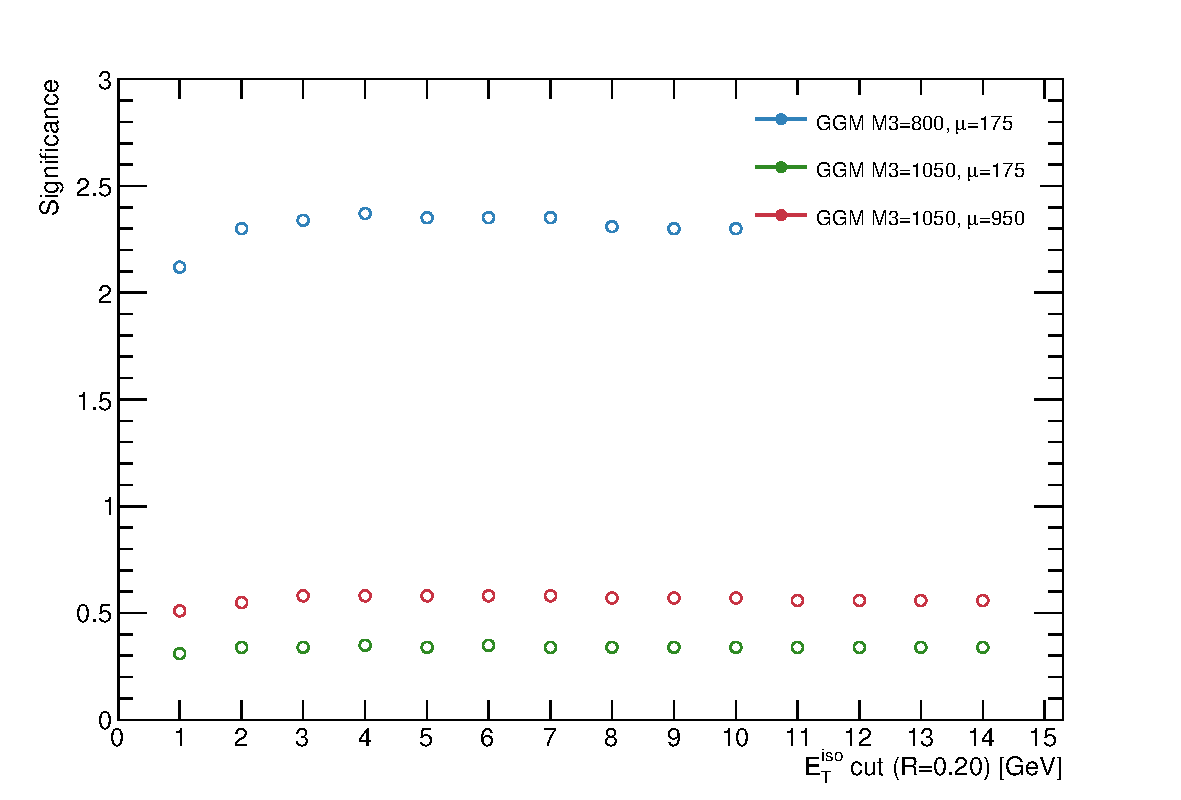
\includegraphics[width=0.3\textwidth]{figures/iso_20_sig}
  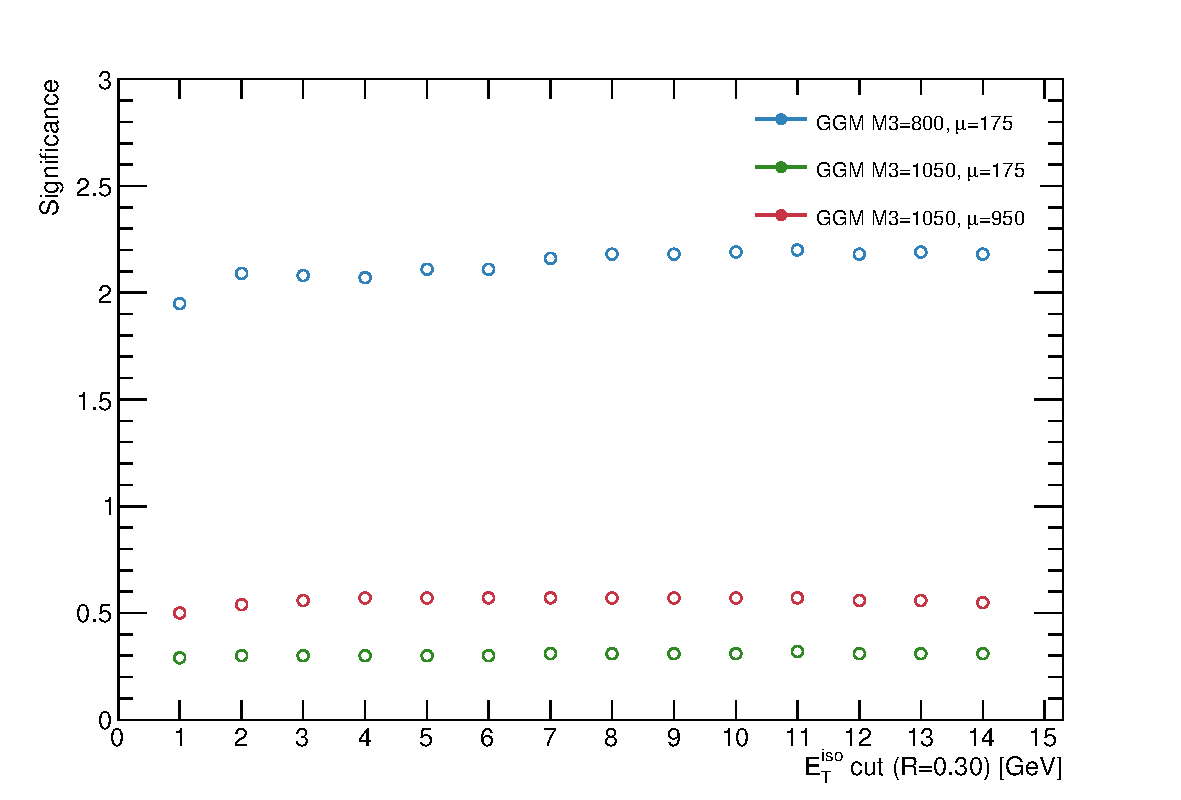
\includegraphics[width=0.3\textwidth]{figures/iso_30_sig}
  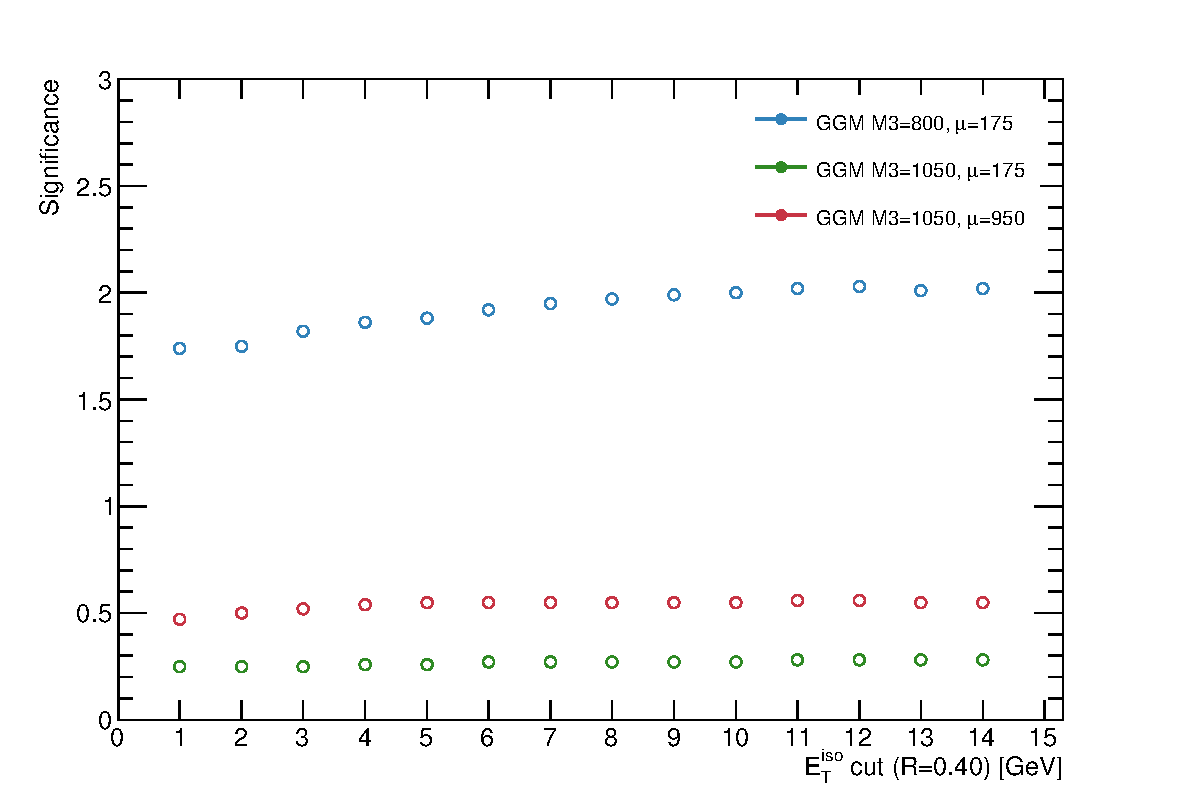
\includegraphics[width=0.3\textwidth]{figures/iso_40_sig}

  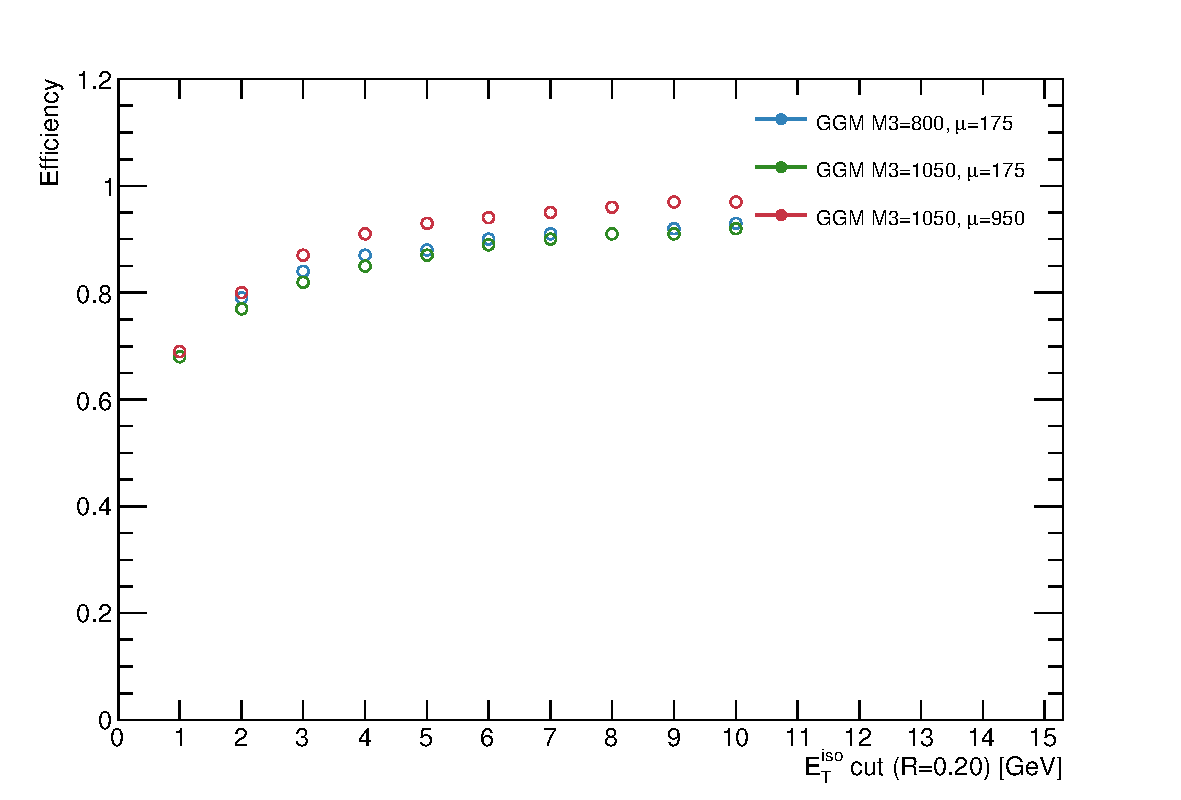
\includegraphics[width=0.3\textwidth]{figures/iso_20_eff}
  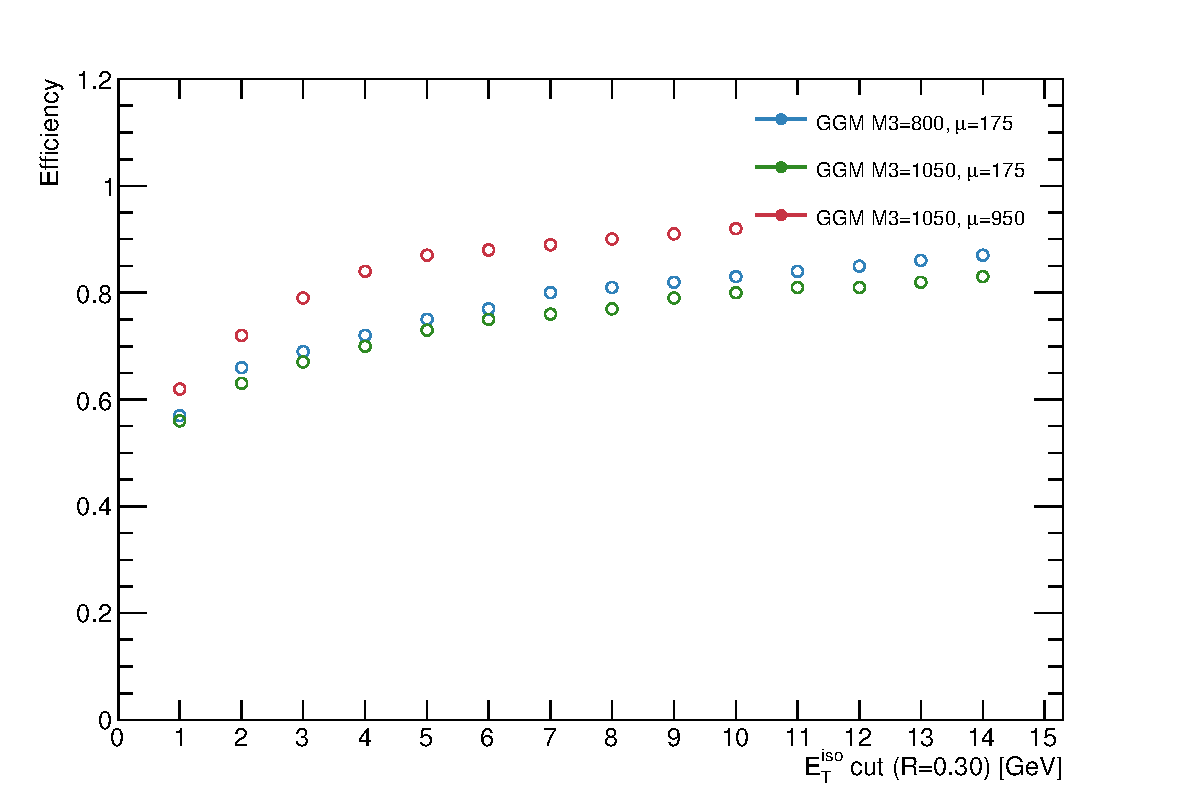
\includegraphics[width=0.3\textwidth]{figures/iso_30_eff}
  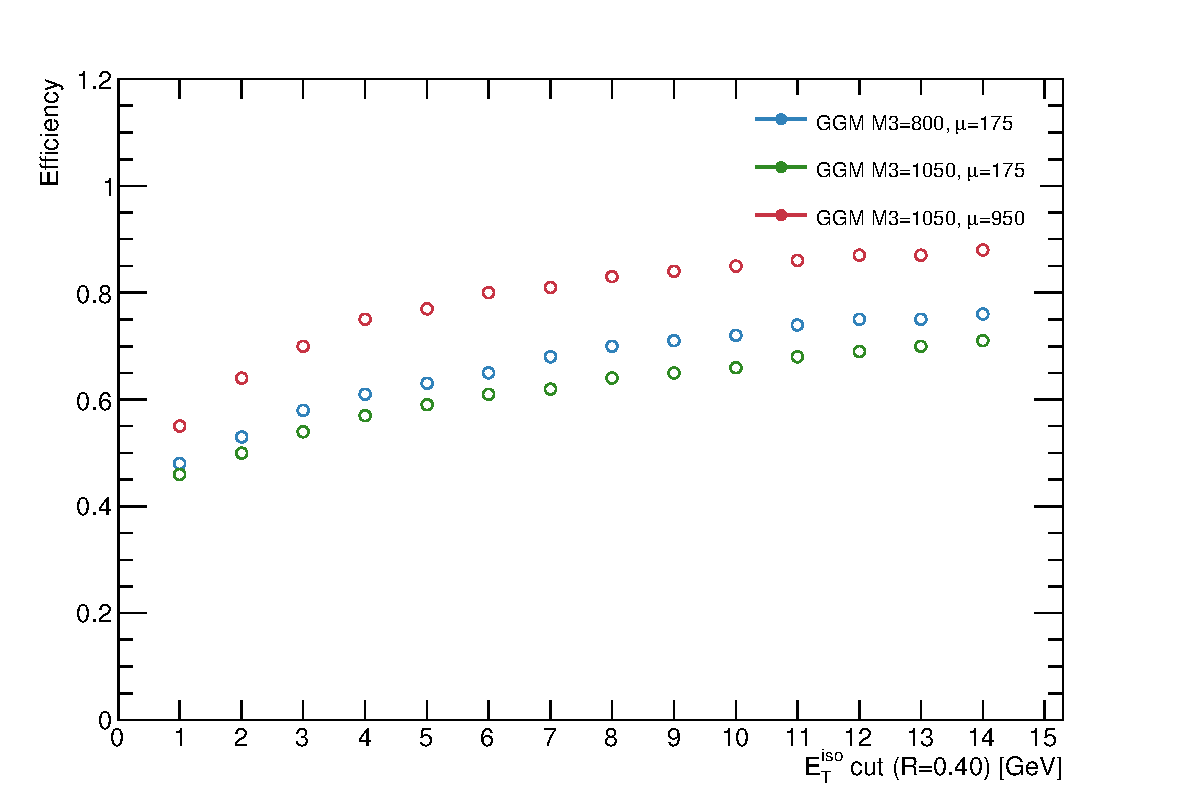
\includegraphics[width=0.3\textwidth]{figures/iso_40_eff}

  \caption{Significancia (arriba) y eficiencia (abajo) vs. el corte en la energía de
    aislamiento, después del corte en {\pt} y {\met}.}
  \label{fig:photon_iso_sig}
\end{figure}


\subsubsection{Leptones y fotones extra}\label{sec:leptonphoton_veto}

Además del veto a los leptones que ya se menciono en la \cref{sec:elec_obj},
los eventos que contengan un segundo fotón con $\pt>75 \gev$, también
son removidos, para mantener las regiones de señal ortogonales al análisis
de dos fotones de ATLAS \cite{ATLAS-CONF-2014-001}.
%% carried out in ATLAS. It is also designed to look for SUSY in
%% GGM scenarios, but particularly sensible to a pure-bino LSP for which the branching ratio to
%% photons is greatly enhanced.

\subsubsection{Energía faltante}

La principal característica de los eventos de SUSY donde se conserva
la paridad-R, es la presencia de una gran cantidad de energía faltante.
Un corte en esta variable reduce enormemente la contaminación de procesos
QCD y también de otros procesos del {\SM}.
La \cref{fig:MET_3SR} muestra la distribución de {\met} en eventos con
un fotón aislado con alto {\pt} (como se definió en la sección anterior),
para tres puntos de señal en cada SR, junto al fondo esperado de simulaciones
MC. Un corte en {\met} relativamente bajo ($> 200 \gev$) es capaz de separar
la señal y el fondo significativamente en {\SRL}, mientras que para {\SRH}
un corte mas alto puede ser aplicado ($>300\gev$).

\begin{figure*}[th!]
  \centering
  \includegraphics[width=0.49\textwidth]{figures/figura} %met_et_SR2}
  \includegraphics[width=0.49\textwidth]{figures/figura} %met_et_SR3}
  \caption{Energía faltante transversa para una luminosidad integrada de {\ilumi}
    luego de que se aplique el corte en el {\pt} del fotón y en la energía de aislamiento
    para {\SRL} (izquierda) y {\SRH} (derecha). }
  \label{fig:MET_3SR}
\end{figure*}


\subsubsection{Multiplicidad y {\pt} de los jets} \label{sec:opt_njet}

La \cref{fig:Njet_3SR} muestra la multiplicidad de jets ($N_{jet}$) para $\pt^{jet} > 40$ \gev,
después de los cortes optimizados en el fotón y la {\met} descriptos anteriormente.
Mientras que la señal tiene típicamente un gran numero de jets, la mayoría de los
fondos W/Z+jets, diboson y QCD se acumulan en la zona de pocos jets. Al menos
dos (cuatro) jets son requeridos para los eventos que pasa la selección de {\SRL} ({\SRH}).
Una mayor multiplicidad es efectivamente esperada para {\SRL} debido a que su objetivo
es la región de gluinos pesados donde el decaimiento dominante es el de producción de
cárganos por un decaimiento de tres cuerpos.

\begin{figure*}[th!]
  \centering
  \includegraphics[width=0.49\textwidth]{figures/figura} %jet_n_SR2}
  \includegraphics[width=0.49\textwidth]{figures/figura} %jet_n_SR3}
  \caption{Numero de jets en la {\SRL} (izquierda) y {\SRH} (derecha) con $\pt > 40 \gev$,
    después del corte en el {\pt} del fotón y {\met}, para una luminosidad integrada de {\ilumi}.}
  \label{fig:Njet_3SR}
\end{figure*}

%{\fig} \ref{fig:jetlead_3SR}  shows the \pt\ of the leading jet, after the photon \pt\ and \etmiss cut,
%and requiring the number of jets to be equal or larger than two for SR1-SR3, and equal or larger than
%four for SR2. Additional signal-background discrimination can be obtained by imposing cuts on the %leading
%jet \pt\ (\pt$(j1)$)since the signal tends to have hard leading jets, in particular for the case involving large
%gluino masses and low to medium neutralino masses (SR2).  For SR1 and SR2 the leading jet \pt\  is %required
%to be larger than 80 \gev~ and 100 \gev, respectively.   After those cuts, in  {\fig} \ref{fig:jetsublead_3SR},
%the subleading jet \pt\  (\pt$(j2)$) distributions for the three signal regions are shown. A further cut is %applied for
%SR1 and SR2, by requiring $\pt(j2)>80$ \gev~  and $> 100$ \gev, respectively.

La \cref{fig:jetlead_3SR} muestra el {\pt} del jet mas energético ($\pt^{j1}$),
después de los cortes descriptos anteriormente. %Adicionalmenteafter the
%% photon \pt, \etmiss\ and $N_{jet}$ requirements described above for each signal region.
%% Additional signal-background discrimination can be achieved by requiring a hard leading
%% jet, particularly for SR2 where the heavy gluinos decay down to relatively light neutralinos.
%% Thus, the leading jet \pt\ in SR2 is required to be larger than 100 \gev. Although a
%% harder requirement is suggested by {\fig} \ref{fig:jetlead_3SR}, it was found better to
%% keep it relatively loose and rely on the shape variables described in sec \ref{sec:shape_vars}.
%% The smaller mass difference between gluino and the lightest neutralino in SR3 leads to a
%% softer jet spectrum and then no further requirement is applied in this region.
%Additional signal-background discrimination can be obtained by imposing cuts on the leading  jet \pt\ since the signal tends to have hard leading jets, in particular for the case involving  large gluino masses and low to medium neutralino masses (SR2).  For SR1 and SR2 the leading jet \pt\  is required to be larger than 80 \gev~ and 100 \gev, respectively.

%% Next, the transverse momentum of the second leading jet ($\pt^{j2}$) was explored,
%% after applying the previous cuts. The distributions for signal and background in
%% each analysis region are shown in {\fig} \ref{fig:jetsublead_3SR}. A further cut
%% is applied for SR2, by requiring $\pt^{j2}>100$ \gev, respectively.

\begin{figure*}[th!]
  \centering
  \includegraphics[width=0.49\textwidth]{figures/figura} %jet1_pt_SR2}
  \includegraphics[width=0.49\textwidth]{figures/figura} %jet1_pt_SR3}
  \caption{Momento transverso del jet mas energético en {\SRL} (izquierda) y {\SRH} (derecha),
    para una luminosidad integrada de {\ilumi}.}
  \label{fig:jetlead_3SR}
\end{figure*}

\begin{figure*}[th!]
 \centering
 \includegraphics[width=0.49\textwidth]{figures/figura} %jet2_pt_SR2}
 \includegraphics[width=0.49\textwidth]{figures/figura} %jet2_pt_SR3}
  \caption{Momento transverso del segundo jet mas energético en {\SRL} (izquierda) y {\SRH} (derecha),
    para una luminosidad integrada de {\ilumi}.}
 \label{fig:jetsublead_3SR}
\end{figure*}

\subsubsection{Ángulo entre jetas y \etmiss}
\label{sec:dphi_obj}

En los eventos de señal, la {\met} es producida por los dos gravitinos.
Se espera por lo tanto que la dirección del {\met} sea aleatoria, sin
estar colacionada con ninguno de los demás objetos del evento.
Por otro lado, si la {\met} es originada de efectos instrumentales o de
neutrinos energéticos en jets, la dirección del {\met} estará correlacionada
con uno de los jets mal medidos. La \cref{fig:jet-MET-phi_3SR} muestra
la separación mínima entre el vector de {\met} y cada uno de los dos jets
mas energéticos, definida como:

%If significant \etmiss arises due to mis-measurement of jet energies,
%backgrounds might be expected to accumulate for which there is only
%a small azimuthal separation between the \ETM vector and the
%direction of a leading or subleading jet. The minimum
%azimuthal angle between \ETM and the direction of
%the leading or subleading jet is defined as

\begin{eqnarray} \label{eq:dphi}
  \min\left[ \cos   \Delta\phi({\rm jet}_{1,2},\MET) \right] &\equiv&  \min \left[\frac{\vec{met} \cdot \vec{p}_{\rm T}^{\rm \; jet,i}}{\met \times \pt^{\rm \; jet,i}}\right] \; \;\; , \;\; i = 1,2
  %cos   \dphijm &\equiv&  min \left[\frac{\ETM \cdot \vec{p}_{\rm T}^{\rm \; jet,i}}{\etmiss \times \pt^{\rm \; jet,i}}\right] \; \;\; , \;\; i = 1,2
  %\Delta \phi_{min}^{jet}
\end{eqnarray}
%

%% after applying the photon \pt, \met, jet {\pt} and multiplicity cuts.
%% A lower bound $\dphijm>0.4$ cut is applied for the two signal regions,
%% which helps to significantly reduce the QCD background and clean events with mis-reconstructed \etmiss.

\begin{figure*}[th!]
 \centering
 \includegraphics[width=0.49\textwidth]{figures/figura} %dphi_jet_met_SR2}
 \includegraphics[width=0.49\textwidth]{figures/figura} %dphi_jet_met_SR3}
 \caption{$\Delta \phi \text{(jet, \MET)}$ para {\SRL} (izquierda) y {\SRH} (derecha)}
 \label{fig:jet-MET-phi_3SR}
\end{figure*}

\subsubsection{Ángulo entre Jet y fotón}

Para regiones del espacio de parametros del modelo de senal
donde los gluinos y los neutralinos tienen alta masa ({\SRH})
un corte en la separacion entre el foton y los jets ayuda a
reducir el fondo, principalmente provieninete de dijets QCD y
fotones prompt, donde un foton (real o falso) tiende a ser
producido en la direccion opuesta al jet mas energetico.
El angulo azimutal entre el foton y el jet principal se define
como:
\begin{eqnarray} \label{eq:dphi}
  \cos \dphijg &\equiv& \frac{\vec{E}_\mathrm{T}^{\gamma} \cdot \vec{p}_\mathrm{T}^\mathrm{jet}}{{E}_\mathrm{T}^{\gamma} \times \pt^\mathrm{jet}}
  %\Delta \phi_{min}^{jet-\gamma}
\end{eqnarray}
%
%% which distribution is shown in {\fig} \ref{fig:jet-photon-phi_SR3},
%% for {\SRH} benchmark signal samples after all previous selection.
%% The cut value chosen for this high gluino-neutralino mass region is $\dphijg<2$.

 % shows the jet-photon $\phi$ separation for signal and backround in SR3, after applying the photon \pt\ ,  \etmiss,  jet  \pt\  and multiplicity as well as  $\Delta \phi \text{(jet, MET)}$ cuts.  The cut value chosen for jet-photon separation in this high mass signal region  is  $\Delta \phi \text{(jet}, \gamma) >2$.
%%   \begin{figure*}[th!]
%%  \centering
%%    \includegraphics[width=0.49\textwidth]{figures/figura}
%%    \caption{\dphijg\ for {\SRH}, after applying the photon \pt, \met, jet multiplicity, jet \pt\ and \dphijm\ cuts
%%      (See text for details), for an integrated luminosity of 20.3 \ifb.  For illustration,
%%    distributions for three signal points are also shown.}
%% \label{fig:jet-photon-phi_SR3}
%% \end{figure*}

\subsubsection{Energia Transversa (\HT)}
\label{sec:ht_obj}

%% Given the high-mass gluinos produced in the GGM model-space explored in this analysis, the total visible transverse energy
%% is expected to be large. Thus, the observable {\HT} defined as the scalar sum of the transverse energy of all individual visible
%% objects in the final state is generally much larger for these signals than it is in background events. After the lepton veto
%% described in sec \ref{sec:leptonphoton_veto}, {\HT} is effectively defined as:

\begin{eqnarray} \label{eq:htaddition}
\HT  &\equiv& \pt^{\gamma} + \sum_{N_\mathrm{jets}} \pt^\mathrm{jet}
\end{eqnarray}

La \cref{fig:HT_3SR} muestra las distribuciones de {\HT}.
%photon \pt,  \etmiss, jet multiplicity, two leading jets  \pt,   jet-\etmiss\  and jet-photon $\phi$ separation cuts.
%A large \HT\ requirement ($>800 \gev$) helps reducing the remaining SM background in SR3. Given the high mass neutralino, the main contribution to \HT\ is coming from the hard photon in the event.
%particularly,  SR3 as significantly larger hadronic activity is observed in the signal samples.  NO
%Cuts are then applied, requiring \HT  larger than 800 \gev\  for both SRs.

%% For the case of SR2, even larger {\HT} values are expected given
%% the larger gluino-neutralino mass splitting.
%% However, as discussed in the next section, a more effective variable
%% has been found ({\rt}) and therefore no {\HT} cut is applied in this
%% region.

\begin{figure*}[th!]
  \centering
  \includegraphics[width=0.49\textwidth]{figures/figura} %ht_SR2}
  \includegraphics[width=0.49\textwidth]{figures/figura} %ht_SR3}
  \caption{Total transverse energy (\HT) distributions for SR2 (left) and SR3 (right),
    after photon \pt, \etmiss, jet multiplicity, jet \pt\ and angular cuts
    (see text for details), for an integrated luminosity of 20.3 \ifb.  For illustration,
    distributions for three signal points in each signal regions are also shown.}
  \label{fig:HT_3SR}
\end{figure*}

\subsubsection{Variables de forma adicionales}\label{sec:shape_vars}

%% Additionally, several event shape variables have been tested to gain further discrimination between signal and background. For this analysis, we use the {\rtt} and {\rt} observables, defined as follows:

\begin{equation}\label{eq:rt_formula}
  R_{T}^{n_{j}^{\min}} = \frac{\sum_{i=1}^{n_{j}^{\min}}p_{\rm T}^{j_i}}{\sum p_{\rm T}^{j}},
\end{equation}
%% i.e. the ratio of the scalar sum of \pt\ for the required lowest number of jets ($n_{j}^{min}$) and the scalar sum of \pt\ for all jets in the event.%whereas for the denominator it is the total number of jets existing


%% It is evident that the distribution pattern of this variable, as pointed
%% out in \cite{PhysRevD.84.055010}, depends on the multiplicity and hardness of the jets. As shown in previous sections, the SUSY signals here considered are characterized by hard multijet events in a wide region of parameter space. Evenmore, the sub-leading jets are comparatively harder than those in SM background events. In the case when

%% $n_{j}^{min} \sim n_{j}$, which is predominant in the latter,
%% then the numerator and denominator in {\eq} \eqref{eq:rt_formula}
%% are almost identical and hence the ratio is close to unity. For signal processes, with $n_{j}^{min} \ll n_{j}$ and comparatively harder jets, the ratio is mostly distributed way below 1.

\begin{figure*}[th!]
  \centering
  \includegraphics[width=0.49\textwidth]{figures/figura} %rt2_SR3}
  \caption{Distribucion de {\rtt} para {\SRH}}
  \label{fig:RT2_3SR}
\end{figure*}

\begin{figure*}[th!]
  \centering
  \includegraphics[width=0.49\textwidth]{figures/figura} %rt4_SR2}
  \caption{Distribucion de {\rt} para {\SRL}}
  \label{fig:RT4_3SR}
\end{figure*}

La \cref{fig:RT2_3SR} muestra la distribucion de rt2 para {\SRH},
despues de la seleccion previa con $n_{j}^{min}=2$. % the photon \pt,  \etmiss, jet multiplicity ($\geq 2$), leading and subleading jet transverse momentum and angular cuts.
La \cref{fig:RT4_3SR} muestra la distribucion de {\rt} para {\SRL},
despues de la seleccion previa $n_{j}^{min} = 4$.
Teniendo en cuenta estas distribuciones, un corte $\rt < 0.85$ para {\SRL}.
%% The lower jet multiplicity for signal events in SR3, makes the signal rt2 distribution
%% more QCD-like, and therefore no background rejection is possible for an acceptable efficiency loss.
%can see that, for the case of SR2, if we discriminate $R_{T}^{4}<0.85 $, a significant fraction of backgrounds can be eliminated with a little effect on the signal efficiency.

%\tosolve{how much? Same for other selection cuts!}.


\section{Selección Final}\label{sec:signal_regions}

Como resultado del proceso de optimización descripto en la sección anterior,
se definen dos regiones de señal:

%% \begin{itemize}\itemsep0.1cm
%% \item[{\bf {\SRL}}] aimed at detecting events in which high mass gluinos are produced, eventually decaying to low to moderate-massed neutralinos. These events are characterized by relatively high energy objects and large multiplicity of hard jets.
%% \item[{\bf {\SRH}}] aimed at detecting events in which high mass gluinos are produced, decaying into moderate to high-mass neutralinos (i.e. low $\Delta m$). These events are characterized by high energy scales.
%% \end{itemize}

Los eventos en cada región son seleccionados con los cortes descriptos en
\cref{tab:sr2} y \cref{tab:sr3}.

\begin{table}[h!]
  \centering
  \caption{Selección para las regiones de señal y sus correspondientes regiones de control.}
  \begin{tabular}{rccccc}
    \hline \hline
                                          &    SR2 &   CRM2 &      CRLW2 &      CRLT2 \\ % &                 VRMX2 \\
    \hline
    $\pt(\gamma_1)$ (\gev) $>$            &    125 &    125 &        125 &        125 \\ % &                   125 \\
    $\pt(\gamma_2)$ (\gev) (if any) $<$   &     75 &     75 &         -  &         -  \\ % &                    75 \\
    N leptons                             &      0 &      0 &          1 &    $\ge 1$ \\ % &                     0 \\
    \met (\gev)                           & $>200$ &  $<50$ &   [100-200] &   [80-200] \\ % & [X-150] (X=50,75,100) \\
    N jets $\ge$                          &      4 &      4 &          4 &          4 \\ % &                     4 \\
    N b-jets                              &      - &      - &          0 &    $\ge 1$ \\ % &                     - \\
    $\pt(j_1)$  (\gev)  $>$               &    100 &    100 &        100 &        100 \\ % &                   100 \\
    $\pt(j_2)$  (\gev)  $>$               &    100 &    100 &        100 &        100 \\ % &                   100 \\
    $\dphijm >$                           &    0.4 &    0.4 &        0.4 &        0.4 \\ % &                   0.4 \\
    $\rt <$                           &   0.85 &   0.85 &          - &          - \\ % &                  0.85 \\
    \hline \hline
  \end{tabular}
\label{tab:sr2}
\end{table}

\begin{table}[h!]
  \centering
  \caption{Selección para las regiones de señal y sus correspondientes regiones de control.}
  \begin{tabular}{rccccc}
    \hline \hline
                                          &    SR3 &    CRM3 &     CRLW3 &    CRLT3 \\ % &   VRH3 \\
    \hline
    $\pt(\gamma_1)$ (\gev) $>$            &    300 &     300 &       150 &      150 \\ % &    300 \\
    $\pt(\gamma_2$) (\gev)  (if any) $<$  &     75 &      75 &       -   &      -   \\ % &     75 \\
    N leptons                             &      0 &       0 &         1 &  $\ge 1$ \\ % &      0 \\
    \met (\gev)                           & $>300$ &   $<50$ &  [100-200] & [80-200] \\ % & $>300$ \\
    N jets $\ge$                          &      2 &       2 &         2 &        2 \\ % &      2 \\
    N b-jets                              &      - &       - &         0 &  $\ge 1$ \\ % &      - \\
    $\pt(j_1)$ (\gev)  $>$                &     40 &      40 &        40 &       40 \\ % &     40 \\
    $\pt(j_2)$ (\gev)  $>$                &     40 &      40 &        40 &       40 \\ % &     40 \\
    $\dphijm >$                           &    0.4 &     0.4 &       0.4 &      0.4 \\ % &    0.4 \\
    $\dphijg <$                          &    2.0 &     2.0 &       2.0 &      2.0 \\ % &    2.0 \\
    \HT (\gev)                            & $>800$ & $> 800$ &         - &        - \\ % & $<800$ \\
    \hline \hline
  \end{tabular}
\label{tab:sr3}
\end{table}


El número de eventos esperado de fondos el {\SM} de las muestras simuladas
después de la selección completa se muestran en la \cref{tab:mc_events_sr1}.
%,\ref{tab:mc_events_sr2},\ref{tab:mc_events_sr3}, for SR1, SR2 and SR3, respectively.
También se presenta el numero de eventos esperado y la significancia para tres puntos
de señal relevantes en cada región de señal.

Se puede ver que la contaminación dominante viene de {\wgam} y {\ttgam}. Adicionalmente
en la \cref{tab:mc_events_sr_phtype} se puede ver el numero de eventos de fondo
esperado separando fotones reales de los eventos donde un jet o un electrón es confundido
con un fotón. El primero tipo de eventos es claramente dominante en este análisis, en
presencia de energía faltante tanto real como instrumental.

La significancia esperada en la grid de señal completa se puede ver en la \cref{fig:opt_exp_significance},
incluyendo el mejor valor de ambas regiones. Es importante notar que estos
resultados son preliminares y obtenidos de simulaciones Monte Carlo. Los resultados
finales son derivados utilizando los métodos de estimación de fondos descriptos en
el \cref{cap:fondos}. %%, y luego del procedimiento descripto en nd after the fitting procedure detailed in \cref{sec:fitresults}.

\begin{table}[!h]
  \centering
  \caption{Número de eventos esperado para los fondos del {\SM}
    y algunos puntos de senal despues de cada corte de la region
    de senal, para una luminosidad integrada de {\ilumi}. La
    significancia esperada para cada punto de senal es tambien
    mostrada.}
  \resizebox{\textwidth}{!}{
    \begin{tabular}{ccccccccccc}
      \hline
                & GGM   &    GGM    &    GGM  & & & & & & & Total\\
      {\bf \SRL}   & (1050,175) & (1150,175) & (1150,650) &  W/Z + $\gam$ & Diboson & W/Z + jets & QCD & \ttbar & \ttbar\gam & background \\
      \hline \hline
      Single Photon                    & 3696.00 & 3671.03 & 50.52 & 29378.86 & 297.09 & 12694.40 & 3392496.25 & 344.62 & 1820.71 & $3437031.93\pm8506.93$ \\
      Photon \pt                       & 3199.64 & 3177.24 & 49.51 & 25195.24 & 230.19 & 10093.10 & 2826296.25 & 251.46 & 1585.17 & $2863651.40\pm7748.67$ \\
      Leptons veto                     & 2903.73 & 2890.27 & 34.74 & 22215.54 & 166.08 & 7808.01 & 2824994.75 & 204.99 & 1084.30 & $2856473.68\pm7725.42$ \\
      N jets                           & 106.54 & 93.15 & 24.99 & 1976.64 & 15.38 & 172.66 & 82028.19 & 66.49 & 518.61 & $84777.97\pm3059.93$ \\
      $\pt(j1)$                        & 84.70 & 71.29 & 24.85 & 1749.41 & 14.29 & 142.19 & 69374.30 & 57.86 & 427.33 & $71765.38\pm3019.91$ \\
      $\pt(j2)$                        & 53.55 & 40.39 & 23.38 & 1066.33 & 8.71 & 95.60 & 37144.05 & 34.06 & 240.60 & $38589.36\pm708.87$ \\
      $\Delta \phi(\text{jet}, \met)$  & 44.78 & 33.88 & 20.07 & 828.96 & 7.83 & 68.13 & 28194.02 & 27.88 & 184.41 & $29311.22\pm613.45$ \\
      \met                             & 14.10 & 9.44 & 15.96 & 7.00 & 0.93 & 0.00 & 2.52 & 1.83 & 4.36 & $16.64\pm3.51$ \\
      $R_T^4$                          & 8.16 & 4.59 & 10.45 & 0.13 & 0.00 & 0.00 & 0.00 & 0.16 & 0.52 & $0.81\pm0.24$ \\
      \hline \hline
      Significance & 4.83 & 3.18 & 5.73 &  &  &  &  &  &  &  \\
      \hline \hline
      \\
      \\
        \hline
            & GGM   &    GGM    &    GGM  & & & & & & & Total \\
        {\bf SRH} & (1050,750) & (1050,950) & (1250,1150) & W/Z + \gam & Diboson & W/Z + jets & QCD & \ttbar & \ttbar\gam & background \\
        \hline \hline
        Single Photon                   & 86.56 & 46.21 & 4.13 & 29378.86 & 297.09 & 12694.40 & 3392496.25 & 344.62 & 1820.71 & $3437031.93\pm8506.93$ \\
        Photon \pt                      & 51.92 & 36.14 & 3.60 & 1152.74 & 6.86 & 153.18 & 57617.59 & 0.73 & 98.96 & $59030.06\pm291.10$ \\
        Leptons veto                    & 41.75 & 34.57 & 3.47 & 1015.11 & 4.40 & 102.50 & 57549.59 & 0.53 & 65.30 & $58737.44\pm286.56$ \\
        N jets                          & 40.86 & 33.20 & 3.28 & 794.99 & 3.36 & 48.81 & 35845.33 & 0.53 & 63.65 & $36756.67\pm222.97$ \\
        $\Delta \phi(\text{jet}, \met)$ & 34.39 & 29.07 & 2.93 & 637.04 & 2.85 & 38.15 & 29026.38 & 0.45 & 45.45 & $29750.33\pm198.00$ \\
        \met                            & 24.28 & 23.17 & 2.46 & 6.01 & 0.23 & 0.00 & 0.83 & 0.04 & 0.59 & $7.70\pm1.09$ \\
        $H_T$                           & 22.20 & 21.26 & 2.34 & 2.52 & 0.01 & 0.00 & 0.83 & 0.04 & 0.24 & $3.64\pm0.68$ \\
        $\Delta \phi(\gam, \text{jet})$ & 14.04 & 13.77 & 1.56 & 0.66 & 0.00 & 0.00 & 0.00 & 0.00 & 0.13 & $0.78\pm0.19$ \\
        \hline \hline
        Significance & 7.05 & 6.96 & 1.37 &  &  &  &  &  &  &  \\
        \hline \hline
      \end{tabular}
  }
  \label{tab:mc_events_sr1}
\end{table}


%%PER PHOTON TYPE
%% \begin{table}[!ht]
  \begin{sidewaystable}[ph!]
    \centering
    \caption{Número de eventos esperado para los fondos del {\SM}
      después de cada corte de la selección de la región de señal
      para una luminosidad integrada de {\ilumi}. Las columnas
      dentro de cada fondo corresponden a fotones reales,
      fotones provenientes de jets y fotones provenientes de electrones,
      respectivamente.}
    \resizebox{\textwidth}{!}{
      \begin{tabular}{rrrr|rrr|rrr|rrr|rrr|rrr|rrr}
        \hline \hline
               {\bf SR2}  & \multicolumn{3}{|c|}{W/Z + \gam} & \multicolumn{3}{|c|}{Diboson} & \multicolumn{3}{|c|}{W/Z + jets} & \multicolumn{3}{|c|}{QCD} & \multicolumn{3}{|c|}{\ttbar} & \multicolumn{3}{|c|}{\ttbar\gam} & \multicolumn{3}{|c}{Total bkg} \\
               & \multicolumn{1}{|c}{$\gamma$} & \multicolumn{1}{c}{$j$} & \multicolumn{1}{c|}{$e$} & \multicolumn{1}{|c}{$\gamma$} & \multicolumn{1}{c}{$j$} & \multicolumn{1}{c|}{$e$} & \multicolumn{1}{|c}{$\gamma$} & \multicolumn{1}{c}{$j$} & \multicolumn{1}{c|}{$e$} & \multicolumn{1}{|c}{$\gamma$} & \multicolumn{1}{c}{$j$} & \multicolumn{1}{c|}{$e$} & \multicolumn{1}{|c}{$\gamma$} & \multicolumn{1}{c}{$j$} & \multicolumn{1}{c|}{$e$} & \multicolumn{1}{|c}{$\gamma$} & \multicolumn{1}{c}{$j$} & \multicolumn{1}{c|}{$e$} & \multicolumn{1}{|c}{$\gamma$} & \multicolumn{1}{c}{$j$} & \multicolumn{1}{c}{$e$} \\
               \hline
               \multicolumn{1}{c|}{Single Photon} & $26129.52$ & $3244.97$ & $4.95$ & $141.72$ & $60.44$ & $94.90$ & $4641.52$ & $3865.33$ & $4058.90$ & $2632820.50$ & $754107.69$ & $0.08$ & $122.01$ & $57.51$ & $164.46$ & $1287.15$ & $532.95$ & $0.56$ & $2665142.41\pm6922.77$ & $761868.90\pm3872.74$ & $4323.84\pm163.11$ \\
               \multicolumn{1}{c|}{Photon \pt}    & $22355.84$ & $2836.87$ & $2.84$ & $109.05$ & $47.27$ & $73.85$ & $3770.90$ & $3101.01$ & $3095.56$ & $2195430.25$ & $624380.69$ & $0.08$ & $88.12$ & $38.47$ & $124.41$ & $1116.70$ & $468.12$ & $0.29$ & $2222870.86\pm6233.56$ & $630872.44\pm3452.89$ & $3297.03\pm140.91$ \\
      \multicolumn{1}{c|}{Leptons veto}  & $19379.52$ & $2833.60$ & $2.76$ & $77.22$ & $34.15$ & $54.69$ & $2997.29$ & $1918.81$ & $2769.29$ & $2194406.50$ & $624106.50$ & $0.08$ & $74.68$ & $25.06$ & $104.94$ & $768.22$ & $315.82$ & $0.22$ & $2217703.43\pm6220.18$ & $629233.95\pm3430.10$ & $2931.98\pm136.77$ \\
      \multicolumn{1}{c|}{N jets}        & $1621.72$ & $354.80$ & $0.12$ & $6.82$ & $5.04$ & $3.52$ & $84.74$ & $38.09$ & $49.84$ & $55224.04$ & $23963.72$ & $0.00$ & $24.05$ & $8.73$ & $33.63$ & $366.01$ & $152.49$ & $0.09$ & $57327.37\pm897.81$ & $24522.87\pm602.64$ & $87.20\pm15.52$ \\
      \multicolumn{1}{c|}{$\pt(j_1)$}    & $1436.19$ & $313.10$ & $0.12$ & $6.55$ & $4.64$ & $3.09$ & $61.91$ & $34.40$ & $45.89$ & $46916.22$ & $19623.34$ & $0.00$ & $21.13$ & $7.25$ & $29.44$ & $305.38$ & $121.86$ & $0.09$ & $48747.38\pm808.73$ & $20104.59\pm528.86$ & $78.63\pm14.79$ \\
      \multicolumn{1}{c|}{$\pt(j_2)$}    & $874.68$ & $191.59$ & $0.06$ & $4.02$ & $2.86$ & $1.83$ & $37.52$ & $28.91$ & $29.16$ & $26512.08$ & $10602.34$ & $0.00$ & $12.54$ & $4.19$ & $17.33$ & $176.60$ & $63.91$ & $0.08$ & $27617.45\pm592.41$ & $10893.80\pm380.87$ & $48.48\pm11.96$ \\
      \multicolumn{1}{c|}{\dphijm}       & $680.66$ & $148.23$ & $0.06$ & $3.57$ & $2.64$ & $1.61$ & $31.65$ & $19.37$ & $17.11$ & $20238.18$ & $7956.02$ & $0.00$ & $10.08$ & $3.44$ & $14.35$ & $135.01$ & $49.32$ & $0.08$ & $21099.16\pm515.51$ & $8179.01\pm326.20$ & $33.22\pm9.20$ \\
      \multicolumn{1}{c|}{\met}          & $7.00$ & $0.00$ & $0.00$ & $0.65$ & $0.17$ & $0.10$ & $0.00$ & $0.00$ & $0.00$ & $2.43$ & $0.09$ & $0.00$ & $0.58$ & $0.54$ & $0.70$ & $3.52$ & $0.84$ & $0.00$ & $14.19\pm3.32$ & $1.65\pm0.46$ & $0.80\pm0.24$ \\
      \multicolumn{1}{c|}{$R_T^4$}       & $0.13$ & $0.00$ & $0.00$ & $0.00$ & $0.00$ & $0.00$ & $0.00$ & $0.00$ & $0.00$ & $0.00$ & $0.00$ & $0.00$ & $0.04$ & $0.00$ & $0.12$ & $0.39$ & $0.13$ & $0.00$ & $0.56\pm0.19$ & $0.13\pm0.05$ & $0.12\pm0.07$ \\
      \\
      \\
      \hline \hline
      {\bf SR3}  & \multicolumn{3}{|c|}{W/Z + \gam} & \multicolumn{3}{|c|}{Diboson} & \multicolumn{3}{|c|}{W/Z + jets} & \multicolumn{3}{|c|}{QCD} & \multicolumn{3}{|c|}{\ttbar} & \multicolumn{3}{|c|}{\ttbar\gam} & \multicolumn{3}{|c}{Total bkg} \\
          & \multicolumn{1}{|c}{$\gamma$} & \multicolumn{1}{c}{$j$} & \multicolumn{1}{c|}{$e$} & \multicolumn{1}{|c}{$\gamma$} & \multicolumn{1}{c}{$j$} & \multicolumn{1}{c|}{$e$} & \multicolumn{1}{|c}{$\gamma$} & \multicolumn{1}{c}{$j$} & \multicolumn{1}{c|}{$e$} & \multicolumn{1}{|c}{$\gamma$} & \multicolumn{1}{c}{$j$} & \multicolumn{1}{c|}{$e$} & \multicolumn{1}{|c}{$\gamma$} & \multicolumn{1}{c}{$j$} & \multicolumn{1}{c|}{$e$} & \multicolumn{1}{|c}{$\gamma$} & \multicolumn{1}{c}{$j$} & \multicolumn{1}{c|}{$e$} & \multicolumn{1}{|c}{$\gamma$} & \multicolumn{1}{c}{$j$} & \multicolumn{1}{c}{$e$} \\
      \hline
      \multicolumn{1}{c|}{Single Photon} & $26129.52$ & $3244.97$ & $4.95$ & $141.72$ & $60.44$ & $94.90$ & $4641.52$ & $3865.33$ & $4058.90$ & $2632820.50$ & $754107.69$ & $0.08$ & $122.01$ & $57.51$ & $164.46$ & $1287.15$ & $532.95$ & $0.56$ & $2665142.41\pm6922.77$ & $761868.90\pm3872.74$ & $4323.84\pm163.11$ \\
      \multicolumn{1}{c|}{Photon \pt}    & $1012.15$ & $140.52$ & $0.07$ & $3.31$ & $2.22$ & $1.32$ & $84.53$ & $34.98$ & $33.68$ & $45115.09$ & $12454.92$ & $0.00$ & $0.20$ & $0.11$ & $0.41$ & $72.60$ & $26.35$ & $0.01$ & $46287.89\pm256.05$ & $12659.10\pm133.23$ & $35.49\pm10.67$ \\
      \multicolumn{1}{c|}{Leptons veto}  & $875.00$ & $140.04$ & $0.07$ & $2.59$ & $1.21$ & $0.61$ & $67.11$ & $11.28$ & $24.10$ & $45062.91$ & $12439.22$ & $0.00$ & $0.17$ & $0.04$ & $0.31$ & $47.88$ & $17.42$ & $0.01$ & $46055.67\pm253.94$ & $12609.21\pm128.09$ & $25.10\pm8.88$ \\
      \multicolumn{1}{c|}{N jets}        & $666.78$ & $128.18$ & $0.04$ & $2.01$ & $0.84$ & $0.51$ & $28.09$ & $7.53$ & $13.19$ & $27263.23$ & $8434.83$ & $0.00$ & $0.17$ & $0.04$ & $0.31$ & $46.62$ & $17.03$ & $0.01$ & $28006.91\pm194.75$ & $8588.45\pm104.80$ & $14.05\pm6.75$ \\
      \multicolumn{1}{c|}{\dphijm}       & $533.09$ & $103.91$ & $0.04$ & $1.51$ & $0.84$ & $0.49$ & $17.43$ & $7.53$ & $13.19$ & $22097.03$ & $6931.89$ & $0.00$ & $0.17$ & $0.00$ & $0.28$ & $33.37$ & $12.07$ & $0.01$ & $22682.61\pm171.23$ & $7056.24\pm95.13$ & $14.00\pm6.74$ \\
      \multicolumn{1}{c|}{\met}          & $6.01$ & $0.00$ & $0.00$ & $0.22$ & $0.01$ & $0.00$ & $0.00$ & $0.00$ & $0.00$ & $0.71$ & $0.12$ & $0.00$ & $0.00$ & $0.00$ & $0.04$ & $0.48$ & $0.11$ & $0.00$ & $7.42\pm1.02$ & $0.24\pm0.15$ & $0.04\pm0.04$ \\
      \multicolumn{1}{c|}{$H_T$}         & $2.52$ & $0.00$ & $0.00$ & $0.00$ & $0.01$ & $0.00$ & $0.00$ & $0.00$ & $0.00$ & $0.71$ & $0.12$ & $0.00$ & $0.00$ & $0.00$ & $0.04$ & $0.19$ & $0.05$ & $0.00$ & $3.42\pm0.61$ & $0.18\pm0.13$ & $0.04\pm0.04$ \\
      \multicolumn{1}{c|}{\dphijg}      & $0.66$ & $0.00$ & $0.00$ & $0.00$ & $0.00$ & $0.00$ & $0.00$ & $0.00$ & $0.00$ & $0.00$ & $0.00$ & $0.00$ & $0.00$ & $0.00$ & $0.00$ & $0.11$ & $0.02$ & $0.00$ & $0.76\pm0.18$ & $0.02\pm0.02$ & $0.00\pm0.00$ \\
      \end{tabular}
    }
  \label{tab:mc_events_sr_phtype}
  \end{sidewaystable}
%% \end{table}


\begin{figure*}[hb!]
  \centering
  \includegraphics[width=0.49\textwidth]{figures/figura} %significance_sr2}
  \includegraphics[width=0.49\textwidth]{figures/figura} %significance_sr3}
  \includegraphics[width=0.49\textwidth]{figures/figura} %significance_best}
  %% \caption{Expected significance for each point in the $M_3-\mu$ grid for SR2 (top left), SR3 (top right).
  %%   The plot at the bottom shows the best significance for each point. These numbers were used just for optimisation purposes and rely on MC expectations for the SM backgrounds. See text for details.}
  \label{fig:opt_exp_significance}
\end{figure*}


%\subsubsection{Acceptance and efficiency}

%% The acceptance $\times$ efficiency ($A\times\epsilon$) was explored for two signal regions at the truth level,
%% to ensure that the optimization procedure does not lead to uncovered regions of the parameter space nor causes
%% abrupt drops in selection efficiency. As seen in {\fig} \ref{fig:efficiency}, no artifacts are observed and a
%% good coverage is expected. The values for $A\times\epsilon$ are tabulated in App \ref{sec:ap:ggm_acceff}.

\begin{figure*}[h!]
  \centering
  \includegraphics[width=0.49\textwidth]{figures/figura} %acceptance_sr2}
  \includegraphics[width=0.49\textwidth]{figures/figura} %acceptance_sr3}
  \caption{Acceptance $\times$ efficiency for each point in the $M_3-\mu$ grid for SR2 (left) and SR3 (right).}
  \label{fig:efficiency}
\end{figure*}


%\section{Regiones de Control}\label{sec:CRs}

%The control regions used in the analysis are listed in {\tab} \ref{tab:CRs} and depicted in {\fig} \ref{fig:CRVRSR}. There are 2 CRs associated with each SR. Each CR$_i$ (i=1,2,3) selection is designed to enhance the population of one of the main backgrounds in the associated SR$_i$ (QCD, W($\to \ell\nu$)/Z($\to \ell\ell$)+\g,
%\ttbar+\g). Any other contamination is either taken from MC (Dibosons, Z($\nu\nu$+jets/\g)) or estimated with the data-driven techniques described in sec \ref{sec:background_estimation}.
%The control regions used in the analysis are listed in {\tab} \ref{tab:CRs} and depicted in {\fig} \ref{fig:CRVRSR}.

%% There are three control regions (CR) associated with each SR,
%% designed to enhance the population of the expected %the main%
%% backgrounds in this analysis, {\wgam} (CRLW), {\ttgam} (CRLT)
%% and QCD {\gjet} (CRM) events. The selection details are summarised
%% in {\tab} \ref{tab:sr2} and \ref{tab:sr3}. Any other contamination
%% is either taken directly from MC (\ttgam) %, Dibosons, Z($\nu\nu$+jets/\gam))
%% or estimated with the data-driven techniques described in sec \ref{sec:background_estimation}.

%The contribution from QCD \gjet\ is modeled with the jet smearing method detailed in the sec \ref{sec:jetsmearing}, to emulate the fake \etmiss\ caused by the jet energy mismeasurement.
%% The final estimate for this background is obtained by normalizing the smeared events passing a dedicated selection (CRQ) defined
%% from the corresponding SR by reversing the \dphijm\ cut ($<0.2$) and removing the $R_{T}$ cuts. An intermediate \dphijm\ region between 0.2 and 0.4 is kept for validation purposes.
%% CRQ selects a sample of events with similar kinematics to the SR but enriched in QCD background events. The QCD multijets contamination in this region,
%% estimated with the ratio method explained in sec \ref{} is explicitly removed from the selected sample to avoid double counting in the global fit
%% described in sec \ref{sec:fitconfig}.
%% The final estimate for the prompt photon background is obtained by normalizing the Sherpa MC events passing a dedicated selection (CRM) defined
%% from the corresponding SR but at low {\met} ($< 50 \gev$). As expected,  CRM selects an enriched sample %of events with similar kinematics to the SR but enriched in
%% of QCD background events. The multijet contamination is independently estimated with the ratio method explained in sec \ref{sec:jetfakes}. %, is explicitly removed from the selected sample to avoid double counting in the global fit described in sec \ref{sec:fitconfig}
%% Some intermediate {\met} regions between 50 {\gev} and the SR cut are kept for validation purposes. Given the large jet multiplicty and \MET requirements in SR2 and SR3, respectively, the prompt photon background is
%% expected to be very small in both signal regions. However, its contribution is not negligible in the control and validation regions so it is important to get a good normalization estimate.


%CRLT and CRLW select respectively \ttbargam and \wlnugam events, by requiring a photon, a lepton, jets and \etmiss. A {\it b}-veto(tag) requirement is applied in CRLW(CRLT) to enrich the sample in \ttbargam and \wlnugam events.
% Both CRs use a looser \etmiss selection with respect to the SR value, as otherwise the control region suffers from lack of statistics.

%% The CRLW and CRLT selections aim for {\wgam} and {\ttgam} events, respectively,
%% by requiring a photon, a lepton, jets and \met. A $b$-jet veto requirement
%% is applied in CRLW to reduce
%% the contamination from \ttgam. An orthogonal selection, asking for at least
%% one b-tagged jet is required in CRLT to enhance the population of {\ttgam}
%% event. Looser {\met} and {\ht} cuts %($>80\gev$) is are also applied in both
%% cases to increase statistics. No {\rt} selection is applied for the same reason.
%% The full list of cuts is given in {\tab} \ref{tab:sr2} and \ref{tab:sr3}.

%A similar approach, but requiring the presence of at least 1 b-tagged jet in the event, was studied for the normalisation of the \ttbargam\ MC.
%However, given the lack of statistics in both data and MC for this selection, no meaningful derivation of a scale factor is possible.
%For this reason, we relied on the MC prediction for this background. Several
%Truth-level studies were made to evaluate and take into account the
%systematics uncertainties associated to the particular choices of the \ttbargam simulation parameters (see sec \ref{sec:syst_ttbargamma}).

%% Two control samples are defined from the data to estimate the contamination in the SR of background events by electron or jet fake.
%% %The are the control samples used as inputs for the weighting procedure.
%% In the CSE sample the role of the photon is replaced by a \texttt{medium++} isolated electron and then weighted to get the final estimate
%% in the SR as described in sec \ref{sec:ewbackground}. Similarly, the jet$\to$photon background is obtained by weighting a pseudo-photon
%% sample (CSJ) defined from the SR selection by reversing the ID cuts satisfied by the high-\pt\ photon as explained in sec \ref{sec:jetfakes}.
%% To ensure orthogonality to the signal region, no tight-isolated photon is allowed in the CSJ selection above the SR {\pt} threshold. All selection
%% cuts are summarized in {\tab} \ref{tab:CRdd}.

%\tosolve{add table for CSE/CSJ definitions?}
%Regions CRE and CRJ are used to select a control sample for the electron and jet fakes data-driven methods. They are not constrained by the global likelihood fit used for the final background estimation.

%% \begin{table}[h!]
%%   \centering
%% \caption{Selection cuts for CSE and CSJ regions defined for the data-driven methods applied in this analysis, associated to each SR.}
%% \begin{tabular}{rcccc}
%%     \hline \hline
%%                                                &    CSE2 &     CSJ2 &    CSE3 &   CSJ3 \\
%%     \hline
%%     leading electron $\pt$ (\gev) $>$          &    125  &       -  &    300  &    300 \\
%%     leading pseudo-photon $\pt$ (\gev) $>$     &      -  &     125  &      -  &      - \\
%%     $\pt(\gamma_1)$ (\gev) (if any) $<$        &    125  &     125  &    125  &    125 \\
%%     N leptons                                  &      1  &       0  &      1  &      1 \\
%%     \met (\gev)                                & $>200$  &  $>200$  & $>300$  & $>300$ \\
%%     N jets $\ge$                               &      4  &       4  &      2  &      2 \\
%%     $\pt(j_2)$  (\gev)  $>$                    &    100  &     100  &     40  &     40 \\
%%     $\dphijm >$                                &    0.4  &     0.4  &    0.4  &    0.4 \\
%%     $\rt <$                                &   0.85  &    0.85  &      -  &      - \\
%%     $\dphijg <$                               &     -   &      -   &    2.0  &    2.0 \\
%%     \HT (\gev)                                 &     -   &      -   & $>800$  & $>800$ \\
%%     \hline \hline
%%   \end{tabular}
%% \label{tab:CRdd}
%% \end{table}

%% \section{Validation Region selections}\label{sec:vrs}

%% A further set of event selections are used to check the results of the background estimation procedure. A set of validation regions (VR), depicted in {\fig} \ref{fig:CRVR_Wgamma}
%% and \ref{fig:CRVR_QCD}, were built very close to the SR cuts space. %As detailed in {\tab} \ref{tab:sr2} and \ref{tab:sr3},
%% Intermediate selections (or side-bands) or reversed cuts were set to check the background modelling in orthogonal yet similar regions to the SR:

%% \begin{description}\itemsep0.1cm
%%   \item[{\bf VRMX}] defined as SR but with an intermediate \etmiss\ requirement ($X\gev<\etmiss<150\gev$) with $X = 50,75,100$. The higher bound ensures the region is orthogonal to SR.\\
%%   \item[{\bf VRH}] defined as SR but with an intermediate \HT\ requirement ($400\gev<\HT< 800\gev$). No VRH2 is defined, as there is no explicit \HT\ cut applied for SR2.\\
%%   \item[{\bf VRQ}] defined from the signal region selections but with a reversed \dphijm\ cut ($< 0.4$) to enhance the QCD fake \etmiss\ background. \\
%%   \item[{\bf VRR}] defined from the signal region selections but with a reversed {\rt} cut ($>0.85$) for SR2.\\
%% \end{description}
  %\item[{\bf VRL}] defined as CRLW but removing the bjet veto. \\
  %\item[{\bf VRZ}] as for SR but reverting the second photon veto. The second leading photon is treated as a missing particle (M), to model the kinematically similar contribution from \znunugam events. \tosolve{not yet!}\\

%% \begin{figure}[h!]
%%   \centering
%%   \includegraphics[scale=0.75]{figures/regions_bjets_leptons}
%%   \caption{Control regions defined for the \wgamma\ (CRLW) and \ttbargam\ (CRLT) backgrounds. Here 'lepton' refers to electrons and muons only.}
%%   \label{fig:CRVR_Wgamma}
%% \end{figure}

%% \begin{figure}[h!]
%%   \centering
%%   \includegraphics[scale=0.75]{figures/figura}
%%   \includegraphics[scale=0.75]{figures/figura}
%%   \caption{Control and validation regions designed to enhance and validate the \gam\ + jet background for SR2 (left) and SR3 (right).}
%%   \label{fig:CRVR_QCD}
%% \end{figure}

%% A set of validation regions was also studied to test the validity of the CR$\to$SR extrapolation in the fit. The results and definitions are discussed in
%% sec \ref{sec:vr_extrapolation}.
